\chapter{Introduction: functional magnetic resonance imaging to study the human brain}\label{chap:bigpic}
\markright{{~{\rm \ref{chap:intro}}. Introduction: functional magnetic resonance imaging to study the human brain}\hfill}{}


\minitoc
 
\newthought{Neuroimaging has emerged} as a distinguished data-acquisition and set of  analysis techniques for probing and observing brain activity.
Acquisition of the data goes hand-in-hand with
  statistical analysis methods for analyzing the data, in view of making specific quantifiable claims. These techniques operate at a scale much coarser than that of the \textit{neuron}: one is interested physiological effects which are ultimately aggregates of activity over large population of neurons (see Fig. \ref{fig:neuron}).

In this introductory chapter, we review the relevant theory sufficient to situate my own work in a larger scientific context. Section \ref{sec:fmri} will
focus on imaging the human brain and preprocessing of the collected data and also classical methodologies for analyzing the data.
% , with a focus on the localization of task-based brain activity.
  Section \ref{sec:rsfmri} will present another way of probing brain function,
  namely the study of background activity at rest.


\section{Functional magnetic resonance imaging}
\label{sec:fmri}
Human neuroimaging consists in acquiring ex-vivo
(non-invasively) image data from normal and
diseased human populations.
Several types of functional imaging techniques have been developed. Electro-encephalography (EEG) and magneto-encephalography (MEG) measure the superficial cortical neural activity of the brain with a high temporal resolution. Functional
magnetic resonance imaging (fMRI)~\citep{agawa1990,ogawa1990b} uses strong magnetic fields to measure changes in
oxygen flow in the brain that correlates with synaptic activity in the brain. This technique yields
information on brain structure, variability, and function at high
spatial resolution. Finally, invasive
techniques have been developed such as positron emission tomography (PET) that
relies on a radioactive tracer to track glucose consumption.

\begin{pagefigure}%[!htpb]
  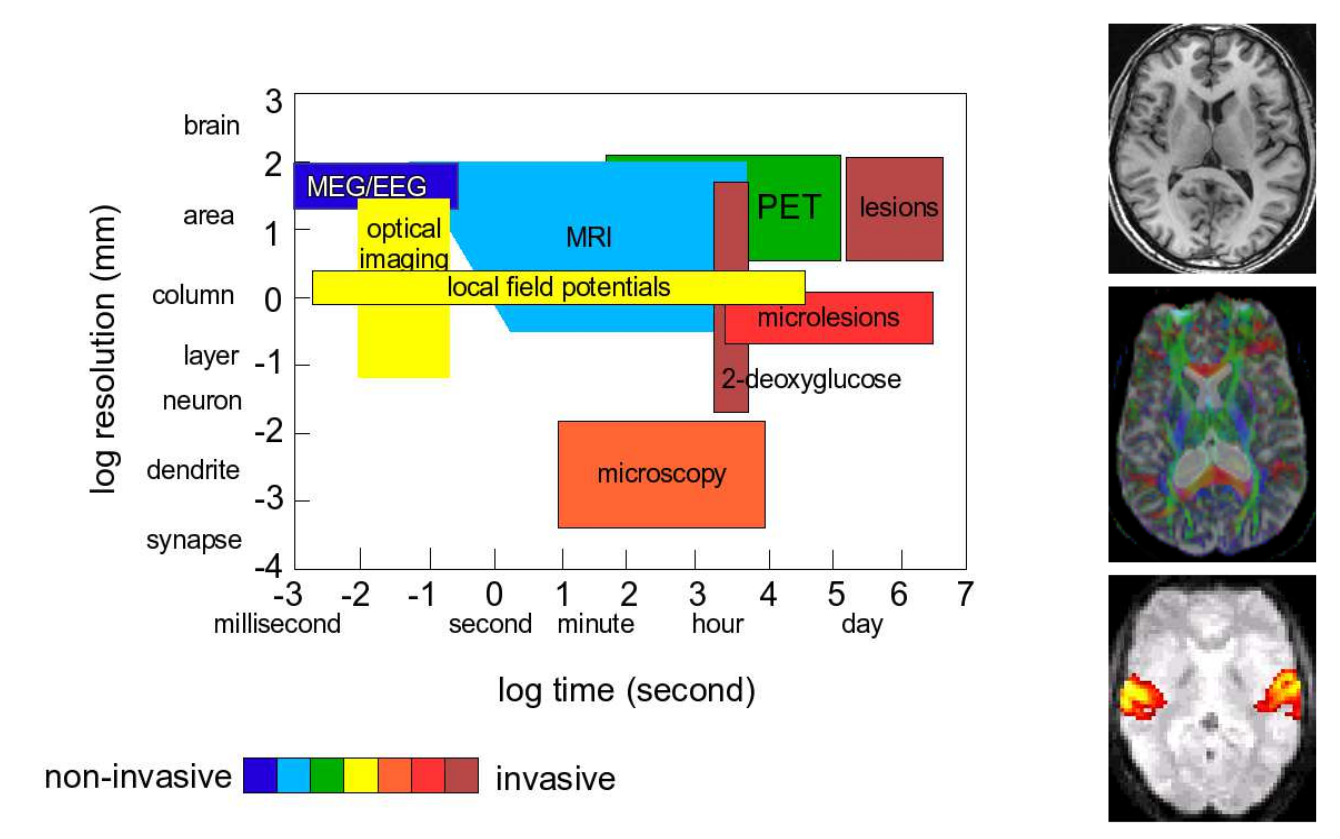
\includegraphics[width=1\linewidth]{figures/modalities.png}
  \caption{\textbf{Imaging modalities} for the brain. \textbf{Left:} The different imaging modalities for brain mapping.
      MRI and functional MRI have
the unique property to yield high-resolution information while being minimally invasive. Unlike other
modalities, MRI allows whole brain imaging. \textbf{Right:} Typical example of T1 / anatomical MRI (top), preprocessed Diffusion-Weighted (DW) MRI \textbf{middle} and fMRI \textbf{bottom} images, presented in axial views.
These images are from the Neurospin 3T scanner. For the DW-MRI image,
the main direction of water diffusion is color-coded: green for antero-posterior diffusion, red for lateral
diffusion, blue for vertical diffusion. The functional image has been analyzed to yield the regions activated
in an auditory task. Adapted with permission from~\citep{thirion_hdr}.}
\end{pagefigure}

\subsection{The BOLD signal}
When a brain area is solicited, the brain fires chemical signals to \textit{report}
the consumption of oxygen and sugar. Nearby blood capillaries dilate to increase the quantity
of flowing blood and provide these resources. This phenomenon is called the
haemodynamic response.
%
As a result, we expect a higher concentration of oxygenated hemoglobin
in a given brain area soon after its activation.
fMRI imaging can be used to measured this effect, called the BOLD (\textit{Blood Oxygen-Level-Dependent}) signal~\citep{agawa1990,ogawa1990b}, at a spatial resolution of 1.5 to 3mm, and a temporal resolution of 1--3s, typically. This yields a spatially resolved image of
brain functional networks that can be modulated
either by specific cognitive tasks or appear as
networks of correlated activity. This method is subject to several physical and physiological
noises. First,
some artifacts may be induced by radio transmitters or other equipment. Then,
spurious activations are naturally introduced by arteries present in
the brain, heart beats and breathing movements. Finally, the brain can be
shifted if the subject makes large movements in the scanner.

\subsection{Preprocessing and analysis of fMRI data}
Raw fMRI images are not intepretable with bare eyes. In particular because
we are interested in small signal co-variation between voxels\footnote{Voxel stands for \textit{volume element}. It refers
to a point in a 3D image, just as pixel refers to a point in a 2D image.}  and not by the
values themselves. The human eye, however, is good at perceiving global artifacts
in the data such as movements, ghost or scanner coils. Quality assessment of
preprocessed fMRI data is done by eye and by relying on dedicated medical
imaging software. In order to prepare the data for further statistical analysis,
some preprocessing steps are required. Below, we outline the main ones. Viz,

\paragraph{Data acquisition.}
The resolution of fMRI is usually between 1mm$^3$ and
(3mm)$^3$ . In a single 3D scan, the brain represents $10^4$ to $10^6$ voxels.
A run contains usually from 100 to 1000 scans. Functional MRI scans are
acquired by slices, usually in the axial direction. The time required to acquire
one slice is called echo time (TE) and is in the order of tens of milliseconds.
The time required to acquire a whole 3D volume is called repetition time (TR)
and is in the order of seconds. Typical values for a 3D volume of 60 slices are
TE=33ms and TR=2s for a 3T (Tesla) scanner.

\paragraph{Motion-correction and coregistration to the anatomy.}
Head movement has a big impact on fMRI. A movement
with an amplitude higher than the voxel resolution (i.e. 2 to 3mm) can
shift the signal of the entire brain. Moreover, the worst impact of motion is
inflow effects, i.e. artefactual signals. In the scanner, the head of the subject is
fixed using cushion pads to avoid movements and the subject is asked to stay
as still as possible. Yet, it is impossible to completely avoid head movement.
In order to mitigate the effect of movement, the 3D scans are realigned on a
reference scan --usually the one in the middle of the sequence-- using rigid
body transformation (translation and rotation, without change of scale).
This is usually followed by an affine registration of the motion-corrected images to
the anatomical (T1) image of the subject, in view of subsequent inter-subject preprocessing and analysis, like registration onto a group template (more on this later).

\begin{figure}[!htpb]
  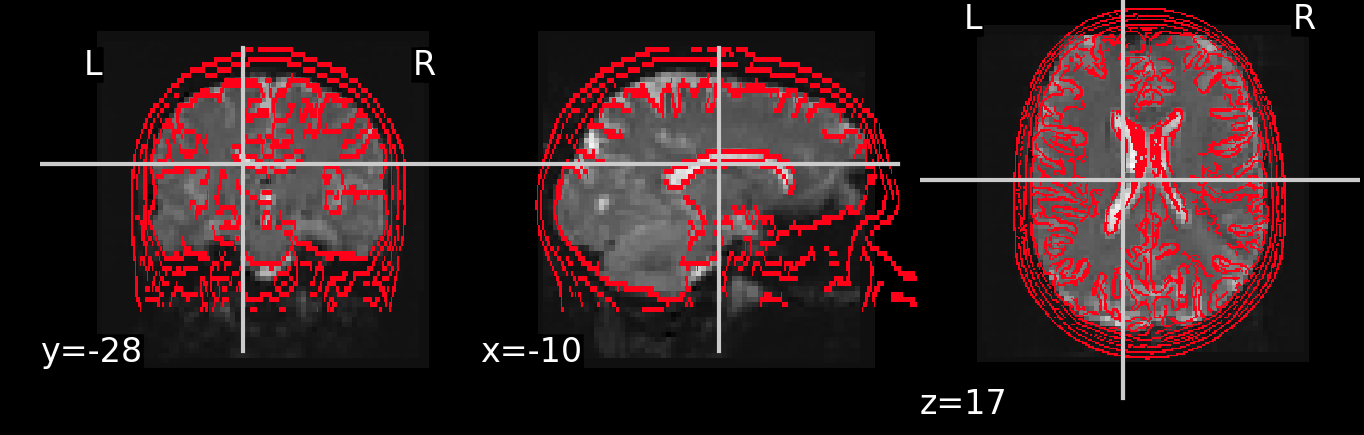
\includegraphics[width=1\linewidth]{figures/coreg.png}\\\\
  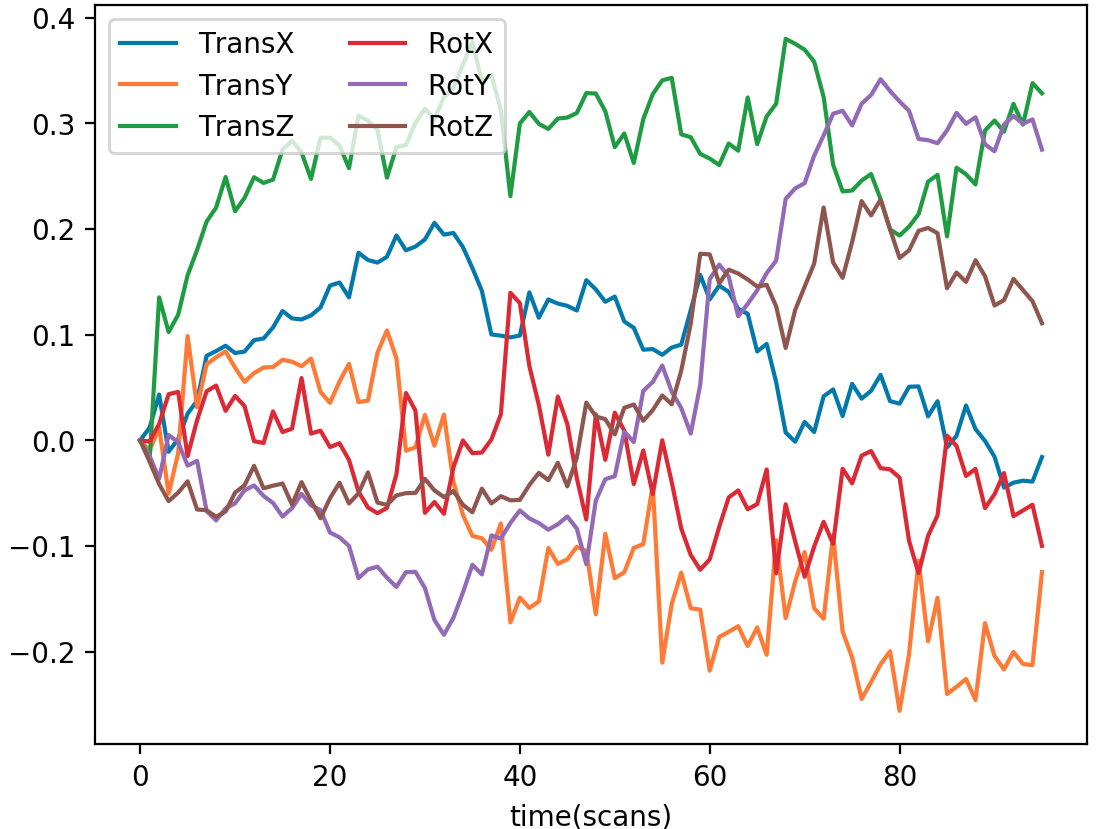
\includegraphics[width=1\linewidth]{figures/mc.png}
  \caption{\textbf{Motion-correction and coregistration.} The \textbf{top} plot shows an overlay of a subjects anatomy onto their mean functional image (the background). Here the red contours are well aligned with the background image, indicative of a successful co-registration. Typical things that can go wrong include: lesions (missing brain tissue), bad orientation headers in the images, non-brain tissue in the images (e.g skull), etc. The \textbf{bottom} plot show estimated motion parameters for the subjects-head motion. Here all movements are well below 0.5mm, which is generally considered as fine. The preprocessing and plots displayed here were done using Pypreprocess ~\url{https://github.com/neurospin/pypreprocess}, an open-source Python wrapper built on standard toolkits like SPM~\citep{friston1994statistical}.}
\end{figure}

\paragraph{Slice-timing correction.}
As stated before, brain slices are not acquired
at the same time. This introduces a shift in the haemodynamic response
associated to each of them. The problem can be solved by interpolating the
signal of each slice so that all of them can be considered as acquired at the
same time. ~\citep{sladky2011} showed that
depending on repetition time and paradigm design, slice-timing effects can significantly impair fMRI results and slice-timing correction methods can successfully compensate for these effects and therefore increase the robustness of subsequent data analysis.

\paragraph{Registration of brain data into a common reference space.}
Each brain is of different size
and shape. In order to compare brain activations across several individuals, we
need to normalize them by registration to a common template~\citep{fristonbook,ashburner2005,ashburner2007,pmid19195496}. This template
can be a reference template used in the community (MNI for example). It is
also possible to compute a template directly from the data. Once a template
is chosen, for each subject, we perform two successive registrations. First,
the anatomical scan acquired in the subject is registered to the MNI template.
Then, the fMRI data are registered to the anatomical scan. After that, the two
transformation matrices are combined in order to normalize the fMRI data to
the template\footnote{In chapter \ref{chap:epi2epi}, we study the possibility of by-passing the anatomical image, when normalizing functional data.}. Estimation of the deformations necessary to warp a subject's brain anatomy onto a template is usually done alongside the classification of individual voxels into different classes: white matter (wm), grey matter (gm), and cerebro-spinal fluid (csf) producing so-called tissue probability maps (TPMs) ~\citep{ashburner2005}.

\begin{figure}
  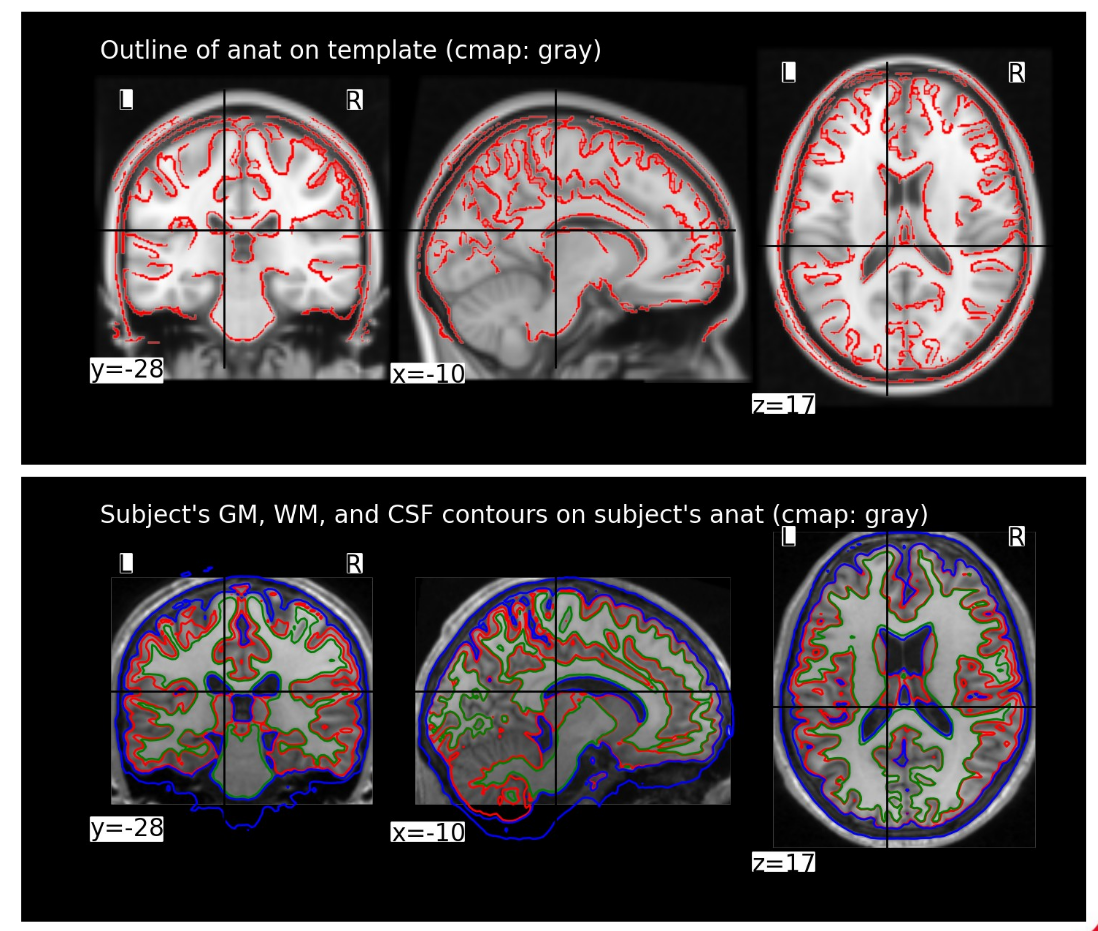
\includegraphics[width=1\linewidth]{figures/normalize.png}
  \caption{\textbf{Tissue segmentation} and \textbf{normalization.} Showing (\textbf{top}) outlines of a subject's anatomical / T1 image (foreground) projected onto an MNI template image (background) and also the tissue probability maps (TPMs), after registration to the latter. The contours should match the background image well. 
% Otherwise, something might have gone wrong.
    Typically impediments to correct registration include:
    lesions (missing brain tissue), corrupted image headers,
non-brain tissue in anatomical image (i.e needs brain
extraction), etc.}
\end{figure}

\subsection{Statistical analysis of brain data}
\label{sec:glm}
Forward inference made on fMRI data (e.g. prediction of brain
activation from the stimuli) can be conceptualized as the \textit{encoding} of perceptual,
motor or cognitive parameters into brain signals. The inverse model, that
predicts behavioral data from brain activation is called \textit{decoding}, and will be the subject matter of chapter \ref{chap:structured_priors}. Two main paradigms allow to experimentally study brain
signals: either we study them in controlled condition on a particular task
--this is the task paradigm-- or we study the spontaneous activity of the brain in
order to uncover its organization: this is the resting-state paradigm.

\subsubsection{The task paradigm and the general linear model}
Using an experimental design, it is possible to relate the BOLD signal with
specific tasks performed by the subject. For example, a sound can be played in
the left or the right ear of the subject. By comparing brain activation between
resting state and when the sound is playing, we can isolate the auditory cortex
of the brain.
Statistically, we do that by crafting a design matrix corresponding to the
experiment: one column of the matrix represents an ideal response to one of the presented conditions~\citep{friston1994statistical}.
Columns corresponding to known artifacts of the BOLD signal, such as heart
beats or movements, can be added in the design matrix in order to regress out
the part of the signal related to them. We then use a general linear model (GLM) to
recover the brain maps corresponding to each of the columns in the design
matrix $\X \in \mathbb R^{T \times k}$, where $k$ is the number of conditions and $T$ is the number of time points (times of repetition -- TR).  It is then supposed that for each voxel $v$, the measured BOLD signal $\y_v \in \mathbb R^T$ is a linear combination of the columns of $\X$, i.e of the experimental conditions, that is

\begin{equation}
  \B{y}_v = \B{X}\boldsymbol{\beta}_v + \boldsymbol{\epsilon}_v,
\end{equation}
where $\boldsymbol{\beta}_v \in \mathbb R^k$ are regression coefficients and $\boldsymbol{\epsilon}_v = (\epsilon_{v,1},\ldots,\epsilon_{v,T}) \in \mathbb R^T$ is a non-iid vector of normally distributed noise.
Such a problem is well-posed and weighted least-squares (WLS) are used to obtain a solution
\footnote{There are usually more time points than experimental conditions, and so the design matrix is full-rank.},
to obtain $\hat{\boldsymbol{\beta}}_v = \B{X}^\dagger\B{y}_v$.  Stacking these coefficients across all voxels per-brain correspond to $k$ so-called $\boldsymbol{\beta}$-maps~\citep{friston1994statistical}. For a given combination of experimental conditions \footnote{For example, for $k = 3$ conditions, one may be interested in take $\B{c} = (1, -1, 0)$, meaning we wish the find the effect of the first condition relative to the second, or $\B{c}=(1,-1/2,-1/2)$ corresponding to the effect of the first condition w.r.t the average effect.\\}
$\B{c}  = (c_1,c_2,\ldots,c_k)\in \mathbb R^k$ , one can compute a statistic

\begin{equation}
\hat{t}_{v,\B{c}} := \frac{\B{c}^T\hat{\boldsymbol{\beta}}_v}{\sqrt{var(\boldsymbol{\epsilon}_v)\B{c}^T(\X^T\X)^{-1}\B{c}}}.
\end{equation}
Under the null hypothesis that the effect were are interested in is zero, i.e
\begin{equation}
  H_0: \B{c}^T\boldsymbol{\beta}_v = 0,
\end{equation}
the above statistic is student-t distributed with $T-k$ degrees of freedom, and one can
analytically obtain $p$-values and confidence intervals for inference. Projecting these values unto the brain (one value per voxel) yields a so-called \textit{activation map}. Such maps are the main output of any forward analysis in task-based fMRI studies.

\begin{figure}
  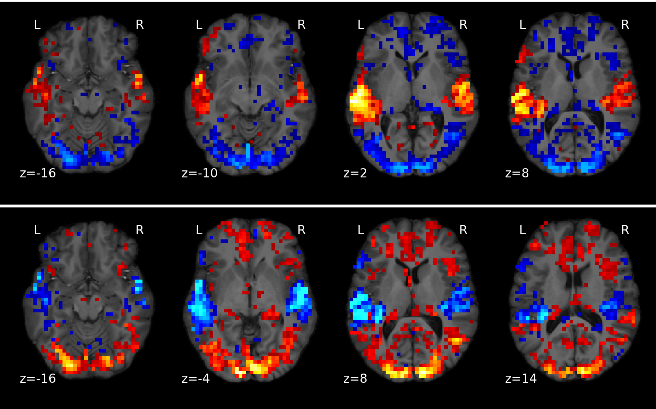
\includegraphics[width=1\linewidth]{figures/activation.png}
  \caption{\textbf{Subject-level Activation maps } for auditory versus visual and visual versus auditory conditions. Here, we show an axial via (z-coordinate) of the Z-values corresponding the size of the effect, in each voxel. Values range from -13 (light blue) to +13 (light red). Analysis was done using the \textit{Nistats} open-source Python library \url{https://github.com/nistats/nistats}.}
\end{figure}

%It should be noted that $T-k$ is only a crude over-estimation of the true degrees of freedom, 
Subsequent statistical inference suffers from heavy \textit{multiple comparison} issues in these so-called \textit{mass-univariate} methods.
%
The problem
is further confounded by the fact that there are correlations between neighboring voxels, leading to  situation where the Bonferoni and similar correction procedures, usually used to deal with these issues, may be too conservative and destroy the the sought-for effects.
%
An alternative is to use \textit{multi-variate} methods which directly model the spatial interactions between the voxels. Such methods will be the subject of chapter \ref{chap:structured_priors}.

\section{Resting-state fMRI, brain networks, and functional connectivity}
\label{sec:rsfmri}
Resting-state fMRI --or rsfMRI for short-- uses the same acquisition method as task fMRI.
However, instead of giving a particular task to the subject, they are asked to let their mind wander without sleeping. By studying this background activity of
the brain, it is possible to uncover its underlying organization~\citep{raichle10}. Unlike the techniques described previously where the aim was to localize regions of activation for a given set of conditions, in functional connectivitly analysis were are interested in infering connections between such regions.

\begin{marginfigure}%[!htbp]
  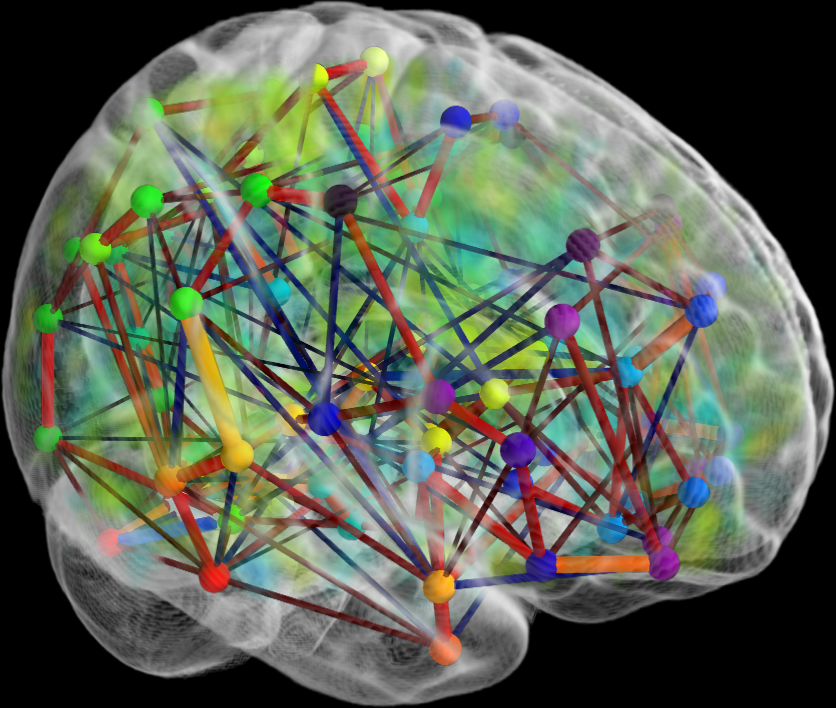
\includegraphics[width=1\linewidth]{figures/connectome.png}
  \caption{\textbf{Functional connectivity} patterns extracted from resting state data. The nodes are regions of the brain, and the thickness
  of the edges represent the relative strength average signal between the two corresponding regions.}
\end{marginfigure}

Depending on the protocol, the subject can be asked to keep eyes closed or
to contemplate a fixation cross. The fixation cross prevents random eye movements
and helps the subject not to sleep.
In rsfMRI, we do not study the signal of each voxel itself but the
interactions between the brain voxels. In particular, we study the functional
connectivity of the brain, i.e. the similarity of activation patterns between
brain regions that share a common functional role. Since there is no design
matrix in rest fMRI, one must be careful to properly regress out physiological
noises or spurious correlations may appear between brain regions, in particular
longitudinally~\citep{power2012,vandijk2012}.
A first approach of functional connectivity is the voxel-to-voxel approach in
which the similarity is measured between each pair of voxels. This method is
not only computationally expensive, given the number of voxels in the brain,
but it is also unfounded from the statistical standpoint: it requires the
estimation of millions of parameters (one for each voxel pair), much more than the number of observations
supports. As a consequence, some form of dimensionality reduction --a feature
selection or extraction-- is necessary to study connectivity.

% \section{Resting-state networks}
% \section{Clinical implications}
% \begin{figure}[!htbp]
%   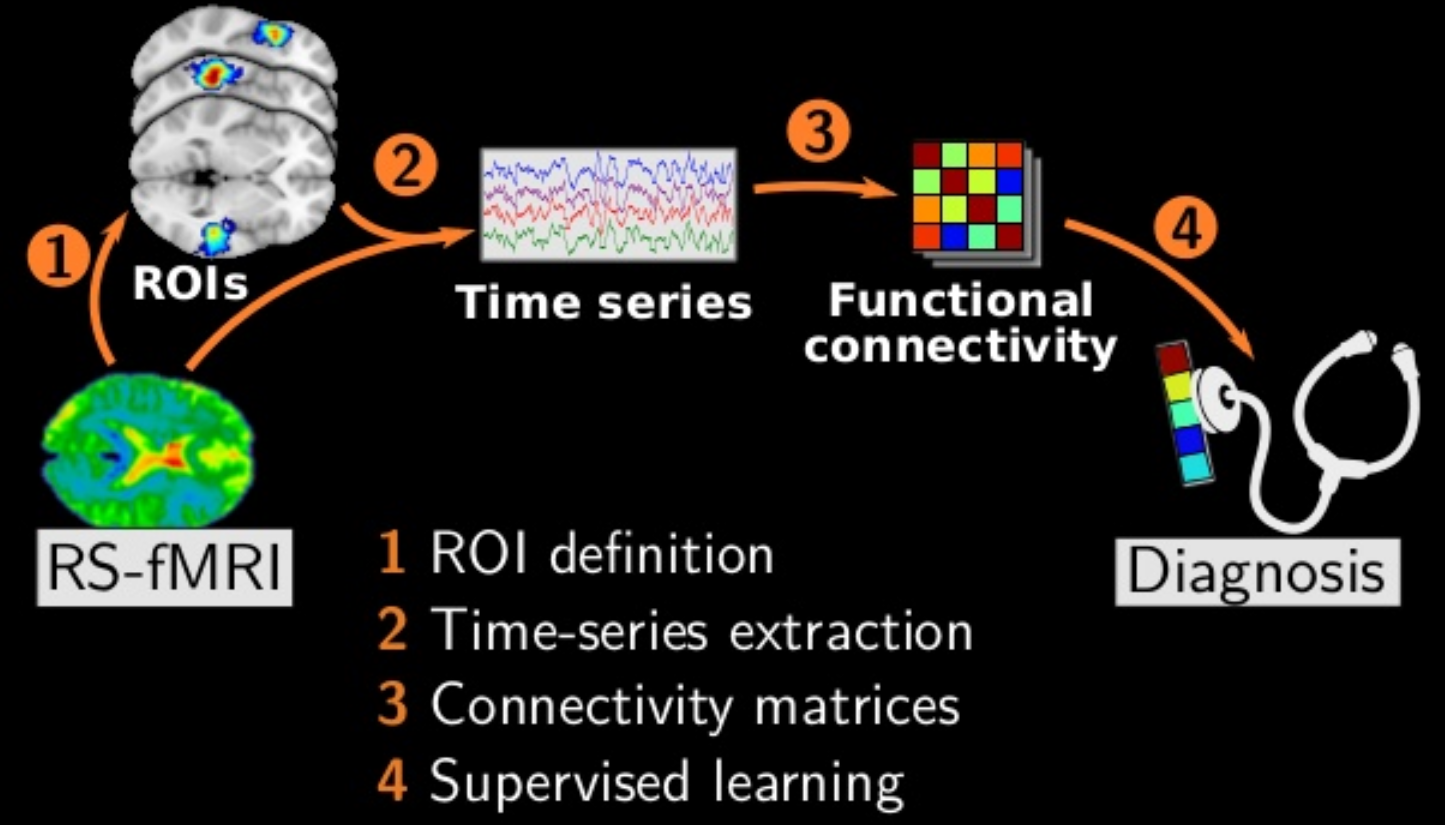
\includegraphics[width=1\linewidth]{figures/big_picture.png}
%   \caption{...}
% \end{figure}
% \section{The functional brain as a dynamic graph}

% \section{Task activation as a small perturbation of resting-state networks}

\section{Inter-subject functional variability}
As noted in
\citep{thirion2007analysis,pmid22425669,Xu2009}, the inter-subject variability
in GLM results is not due to misregistration, but intrinsic subject
differences with a more physiological nature: the size of effects and
the anatomical localization are subject-specific. Also, \citep{tavor2016task} used
dual regression \citep{Filippini2009} to provide quantitative evidence that inter-subject
differences in task-based brain activations are largely physiological --in contrast to being driven
by subjects' brain morphological differences.

Chapters \ref{chap:func_var} and \ref{chap:rsfmri2tfmri} will present generative models for understanding inter-subject variability at the functional level.
% \clearpage
\bibliographystyle{plainnat}
\bibliography{bib_all}
